\subsubsection{FOC-Treiber}
\label{subsubsec:FOC-Treiber_TMC4671}

%Der FOC-Treiber berechnet den Modulationsindex für die Kommutierung der H-Brücke anhand des Drehmoments, der Geschwindigkeit oder der Position, welche der Mikrocontroller dem FOC-Treiber vorgibt. Als Feedback benötigt der FOC-Treiber den momentanen Strom durch zwei der drei Spulen und eine Information über die momentane Lage des Rotors. Die vom FOC-Treiber ausgehenden PWM-Leitungen gehen direkt auf den Gate-Treiber, welcher dann wiederum die MOSFETs ansteuert.
%Der dritte Strom wird mit dem Knotengesetz berechnet. Da der BLDC in Stern geschaltet ist gilt:
%\begin{equation}
%I_U + I_V + I_W = 0
%\end{equation}

Beim FOC-Treiber handelt es sich um den TMC4671. Abbildung \ref{fig:FOC} zeigt die interne Logik des ICs. Kern des FOC-Blocks bildet die Clarke- und Park-Transformation. Die Clarke-Transformation transformiert die drei Teilflüsse (I$_U$, I$_V$, I$_W$) der Spulen im dreiphasigen System zu einem Gesamtfluss im zweiphaseigen System. Die Park-Transformation transformiert die gemessenen Wechselgrössen im stehenden, statorbezogenen Koordinatensystem in einfach regelbare Gleichgrössen im sich drehenden, rotorbezogenen Koordinatensystem. So kann interpretiert werden, wie der Rotor zum Fluss steht. Ziel der FOC-Logik ist, dass der Fluss so ausgerichtet ist, dass nur eine tangentiale Kraft und somit ein Drehmoment auf den Rotor wirkt, was in Abbildung \ref{fig:FOC_2} veranschalicht wird. Im FOC-Block wird dies durch die Null vor dem PID$_D$-Block verdeutlicht. Die Stärke des Drehmoments wird mit dem PID$_Q$-Block geregelt. Die Abweichung ergibt sich durch die Differenz der Eingangssignale auf die PID-Blöcke. Die Blöcke PID$_D$ und PID$_Q$ berechnen anhand der Abweichung eine neue Soll-Spannung, damit der Fluss und somit das Drehmoment gemäss den Sollwerten am Rotor anliegt. Die iPark-Transformation transformiert das sich drehende, rotorbezogene Koordinatensystem zurück in ein stehendes, statorbezogenes Koordinatensystem und die iClarke-Transformation transformiert wiederum das zweiphasige System in ein dreiphasiges System. Anhand dieser Sollspannungen wird von der eingebauten PWM-Engine das Gate-CTRL-Signal erzeugt und an den Gate-Treiber (Power Stage) weitergeleitet.

\begin{figure}[H]
	\centering
	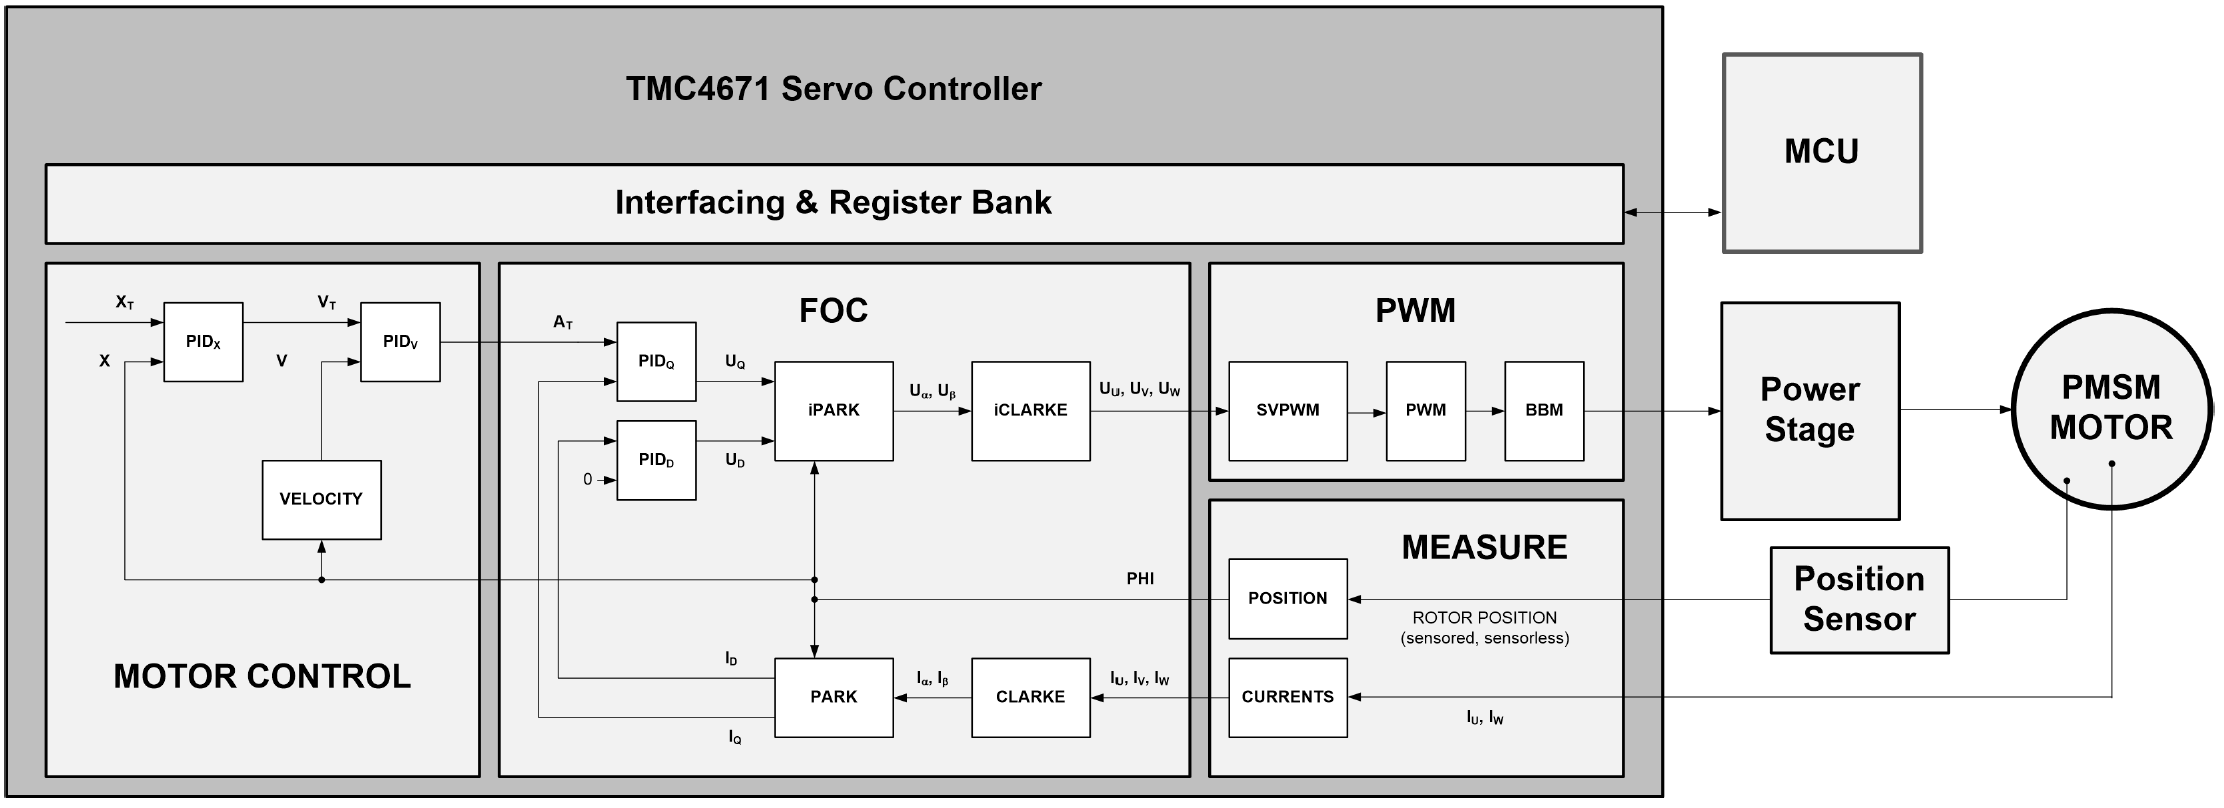
\includegraphics[width=\textwidth]{graphics/FOC}
	\caption{Logik des FOC-Treibers. \cite[S.14]{trinamicmotion_control_gmbh__co_kg_tmc6200_2019}}
	\label{fig:FOC}
\end{figure}

\begin{figure}[H]
	\centering
	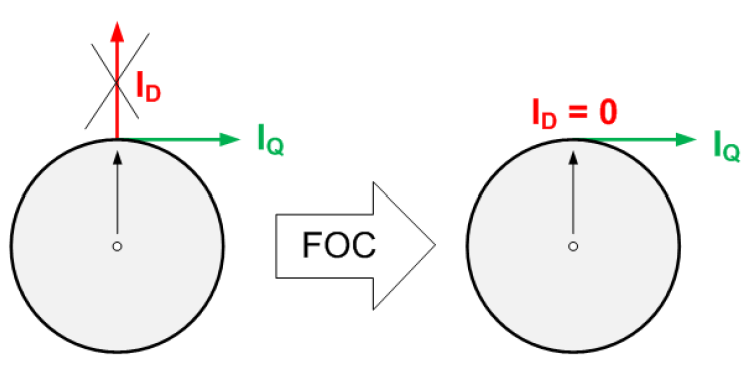
\includegraphics[width=0.4\textwidth]{graphics/FOC_2}
	\caption{Veranschaulichung FOC-Regelung. \cite[S.9]{trinamicmotion_control_gmbh__co_kg_tmc6200_2019}}
	\label{fig:FOC_2}
\end{figure}

Die Sollwerte für die Stärke des Drehmoments kann im Drehmoment-Modus manuell vorgegeben werden oder im Geschwindigkeits- oder Positionsmodus vom überlagerten Geschwindigkeitsregelkreis. Im Gegensatz zu einem Motor, dem nur eine Spannung vorgegeben wird, kann bei diesem Regelverfahren bei einer Abweichung des vorgegebenen Parameters nachgeregelt werden. So kann beispielsweise bei grösserer Belastung die angelegte Spannung erhöht werden, sodass die vorgegebene Geschwindigkeit gehalten werden kann.

Dies führt zur Kaskadenregelung, der PI-Regelstruktur im FOC-Treiber. Eine Kaskadenregelung besteht in der Regel aus drei überlagerten Regelkreisen. Der innerste Regelkreis ist der Stromregelkreis. Dieser ist dem Geschwindigkeitsregelkreis unterlagert. Der Geschwindigkeitsregelkreis ist wiederum dem Positionsregelkreis unterlagert. Bei einer Kaskadenregelung ist die Ausgangsgrösse des überlagerten Regelkreises die Eingangsgrösse des unterlagerten Regelkreises. Aus Stabilitätsgründen ist darauf zu achten, dass die Nachstellzeit der äusseren Regelkreise grösser ist, als die der Inneren.

%Die Regelung im FOC-Treiber besteht im innersten aus einem schnellen Stromregelkreis. Dieser soll in der Lage sein, schnellst möglich auf eine Abweichung des vorgegebenen Drehmoments zu reagieren. Die Abweichung des Stromregelkreises ist ein wichtiger Parameter zur Berechnung des Modulationsindex, welcher der Kommutierung des Motors dient.

%Der Geschwindigkeitsregelkreis ist dem Stromregelkreis überlagert. Weicht die aktuelle Geschwindigkeit von der vorgegebenen Geschwindigkeit ab, so gibt der Geschwindigkeitsregelkreis dem Stromregelkreis eine Abweichung vor, wodurch der Strom durch die Spulen und somit das Drehmoment erhöht oder gesenkt wird.

%Der Positionsregelkreis ist dem Geschwindigkeitskreis überlagert. Weicht die aktuelle Position von der vorgegebenen Position ab, so gibt der Positionsregelkreis dem Geschwindigkeitsregelkreis eine Abweichung vor, wodurch der Geschwindigkeitsregelkreis in die erforderliche Richtung korrigiert.

Mit der Begrenzung der PI-Werte wird die Mechanik geschont und der Motor vor Überlast geschützt. Dies wird erreicht, indem die Ausgangsgrössen der PI-Regler mit einem Limit versehen werden. So kann der Strom durch die Spulen begrenzt werden, eine Maximalgeschwindigkeit definiert werden und die Enden der Positionen vorgegeben werden. Die Limits sind auf den Motor abgestimmt. \cite{stahl_simulation_2014}

\paragraph{Schema}\label{par:Schaltungsaufbau_TMC4671}\mbox{}

Der Treiber und dessen Beschaltung ist als Breakoutboard erhältlich. Daran sind diverse Anschlussmöglichkeiten vorhanden. In Abbildung \ref{fig:Schema_FOC_Treiber} ist erkennbar, welche Pins für den PartyMixer verwendet werden:

\begin{itemize}
\item SPI Input
\item Phasenströme Input
\item Encoder Input
\item Motorspannung Input
\item Gate-CTRL-Signale Output
\end{itemize}

\begin{figure}[H]
	\centering
	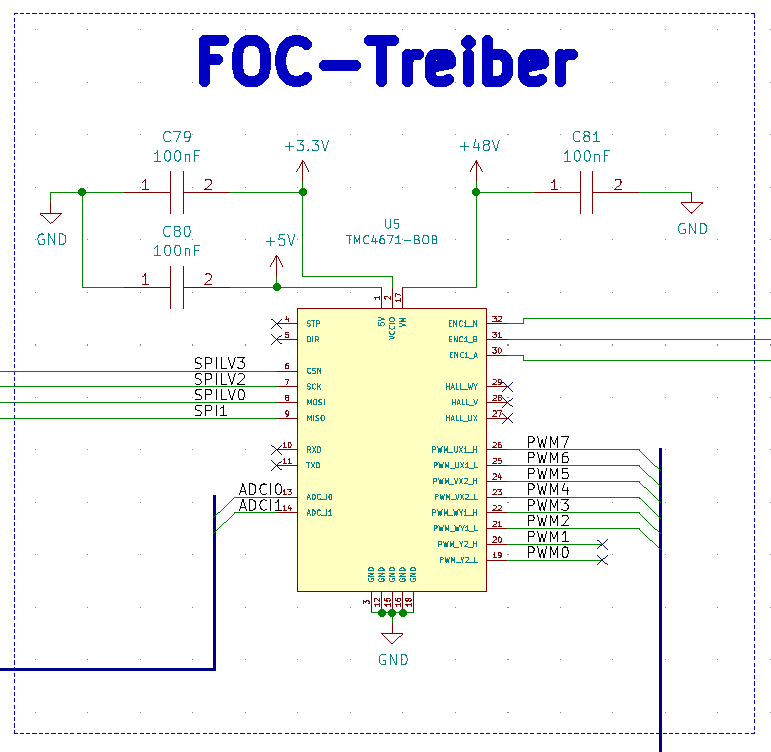
\includegraphics[width=0.7\textwidth]{graphics/Schema_FOC_Treiber}
	\caption{Schema FOC-Treiber.}
	\label{fig:Schema_FOC_Treiber}
\end{figure}

Im Schema sind rote Korrekturen zu sehen. Da das Breakout-Board extern montiert wurde, sind die geshifteten SPI-Leitungen an den Header-Pins nicht belegt und werden deswegen für das externe Breakout-Board des Gate-Treibers verwendet.

\newpage

\paragraph{Funktionsbeschrieb der Schaltung}\mbox{}

%Die Kondensatoren C79 bis C81 in Abbildung \ref{fig:Schema_FOC_Treiber} sind Stützkondensatoren zur Glättung der Versorgungsspannung.

Im Folgenden werden kurz die Teilsysteme auf dem TMC4671-BOB beschrieben. Sämtliche Teilschemas aus dem Datenblatt sind im Anhang Kapitel \ref{Appendix:BOB} aufgezeigt.

%\subparagraph{Kommunikation Input (SPI)}

Der \textbf{SPI}-Kommunikationseingang ist nicht speziell geschützt. Im Layout wurde darauf geachtet, dass die angelegte Spannung nicht über 3.3V steigt. Dies wird mit einem Level-Shifter zwischen Mikrocontroller und FOC-Treiber gewährleistet.

%\subparagraph{Ströme Input (ADC)}

Der Eingang zur \textbf{Strommessung} ist mit einem Tiefpass geschützt. Hier werden hochfrequenze Störsignale, welche auf der Übertragungsstrecke induziert werden, gefiltert. Das Filter hat die Zeitkonstante:

\begin{equation}
\tau = R308 \cdot C300 = 100\Omega \cdot 100pF = 10ns
\end{equation}

%\subparagraph{Encoder Input (ENC)}

Um den Eingang der \textbf{Encoder}-Pins zu schützen, wird ein Schmitt-Trigger mit eingebautem Level-Shifter verwendet. Zudem wird mit dem vorgeschalteten Kondensator- und Widerstandsnetzwerk ein Entprellen der Encoder-Signale erreicht. Wird der Input auf 0V gezogen, so entlädt sich der Kondensator über die Widerstände R200-R202 mit der Zeitkonstante:

\begin{equation}
\tau = R200 \cdot C204 = 1k\Omega \cdot 100pF = 100ns
\end{equation}

Sobald der Eingang vom Encoder nicht mehr auf 0V gezogen wird, so lädt sich der Kondensator über die Widerstände R200-R202 sowie R206,R208,R210. Somit ergibt sich eine längere Zeitkonstante:

\begin{equation}
\tau = (R200 + R210) \cdot C204 = (1k\Omega + 4.7k\Omega) \cdot 100pF = 570ns
\end{equation}

Ohne diese Schaltung kann es vorkommen, dass bei einem schwingenden Signal die Auswertungslogik unabsichtlich einen Schritt misst, ohne dass einer vorgekommen ist. In Abbildung \ref{fig:Schmitt_Trigger_Debounce} ist die Funktion verdeutlicht.

\begin{figure}[H]
	\centering
	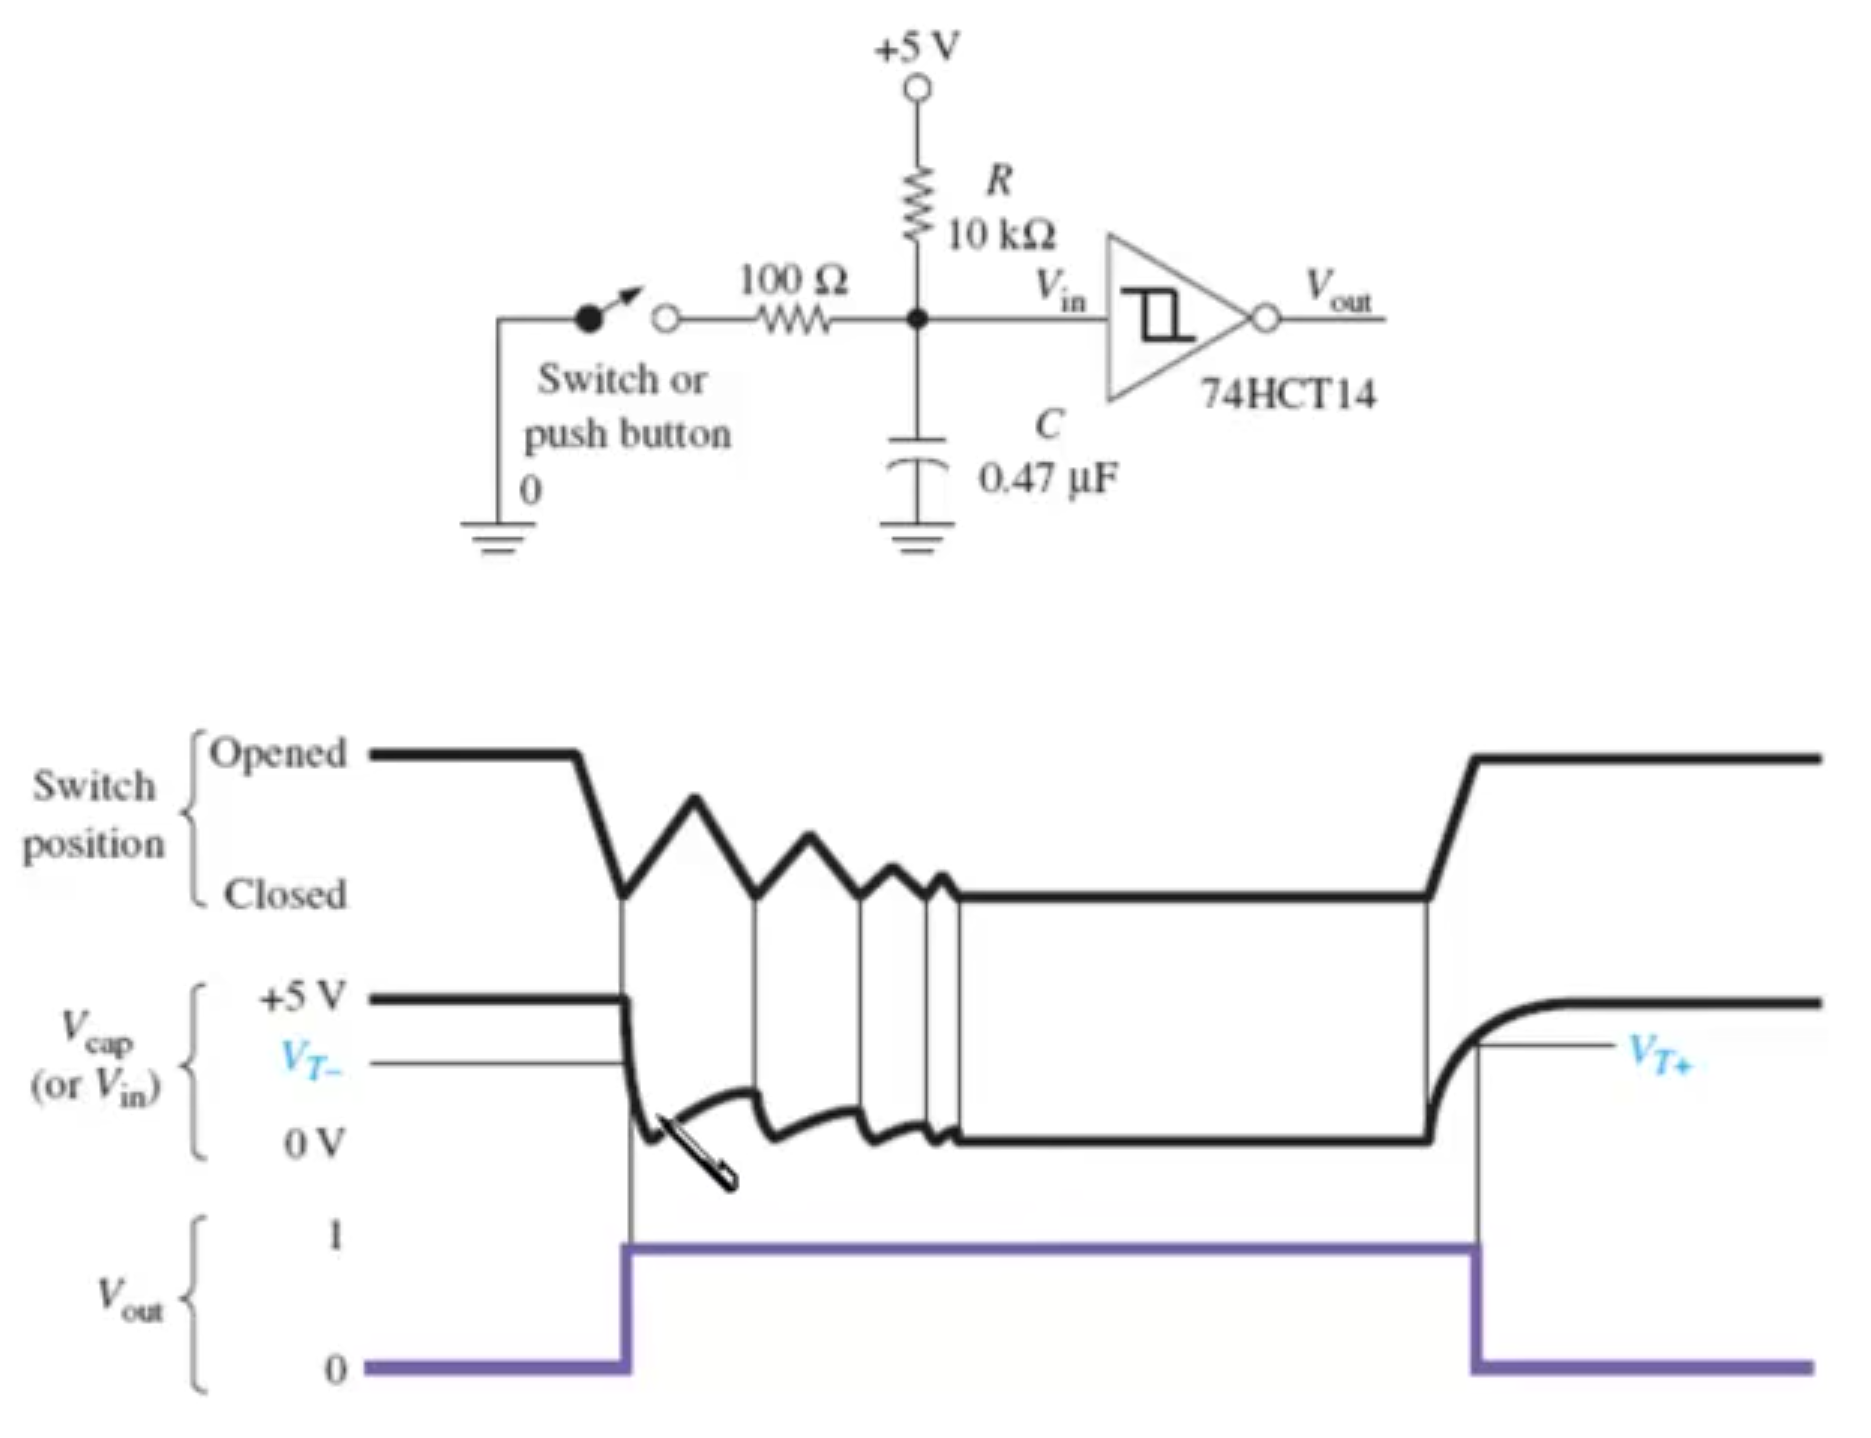
\includegraphics[width=0.7\textwidth]{graphics/Schmitt_Trigger_Debounce}
	\caption{Schmitt-Trigger Debounce-Schaltung. Achtung, die Abbildung entspricht nicht direkt der Schaltung auf dem Breakout-Board, sie dient lediglich der Veranschaulichung. \cite[3:00]{kleitz_sec_2011}}
	\label{fig:Schmitt_Trigger_Debounce}
\end{figure} 

%\subparagraph{Motorspannung Input (48V)}

Die \textbf{Motorspannung} ist wichtig, um den Kommuntierungsvorgang zu berechnen. Wichtiger als die Zeitkonstante ist hier ein Spannungsteiler, welcher die Motorspannung auf unter 3.3V bringt. Dazu wird folgende Formel angewendet:

\begin{equation}
U_{TMC} = U_M \cdot \frac{R310}{R310 + R311} = 48V \cdot \frac{1k\Omega}{1k\Omega + 100k\Omega} = 0.7V
\end{equation}

Ausserdem ergibt sich aus er Schaltung ein Eingangsfilter \cite{andy_aka_capacitor_2013}:
\begin{equation}
\tau = C302 \cdot \frac{R310 \cdot R311}{R310 + R311} = 10nF \cdot \frac{1.5k\Omega \cdot 100k\Omega}{1.5k\Omega + 100k\Omega} = 147us
\end{equation}

%\subparagraph{Gate-Ctrl-Signale Output (PWM)}

Die \textbf{Gate-CTRL-Signale} für den Gate-Treiber gehen direkt auf die Header-Pins des BOBs.

%\subsubsection{Encoder-Input}\label{subsubsec:Encoder_Input}
%
%Vor einem Analogeingang wird das Signal in der Regel mit einem Tiefpass gefiltert, um stochastische Abweichungen zu verhindern. Dafür werden die Widerstände \textbf{R700-R702} und die Kondensatoren \textbf{C700-C702} verwendet. Die Beschaltung und Dimensionierung wurde aus dem Datenblatt des TMC4671-EVAL-Board entnommen. Die Zeitkonstante des Filters beträgt gemäss Formel \ref{equ:Berechnung_Encoder_LP} 10ns. Das Schaltungsprinzip ist in Abbildung \ref{fig:Schema_Encoder_LP} dargestellt. 
%\begin{equation}
%\tau = R \cdot C = 100\Omega \cdot 100\cdot10^{-12}F = 10 \cdot 10^{-9}s = 10ns
%\label{equ:Berechnung_Encoder_LP}
%\end{equation}
%
%Der Motor hat eine Drehzahl von max. 1500rpm, dies entspricht einer maximalen Periodendauer von $\mathrm{666.\overline{6} \mu}$s. Das Eingangssignal wird deshalb nicht herausgefiltert.
%
%Die Komponenten \textbf{D700-D702} sind Bauteile, welche zwei Shottky-Dioden verbaut haben und sind dazu da, eventuell auftretende Über-/ und Unterspannungen zu verhindern. Abbildung \ref{fig:Schema_Encoder_2_LP} zeigt die Anordnung der internen Dioden an Stelle des
%verwendeten Bauteils. Jede Diode hat eine Durchlassspannung von 0.3V. Liegt in Abbildung \ref{fig:Schema_Encoder_2_LP} beim Eingangssignal eine Spannung von über 5.3V an, wird die Diode an 5V leitend und verhindert ein weiteres Ansteigen der Eingangsspannung. Das Selbe bei Unterspannung, sobald eine Spannung von -0.3V anliegt, wird die Diode an 0V leitend, und verhindert ein weiteres Absinken der Spannung.

%\begin{figure}[h!]
%	\centering	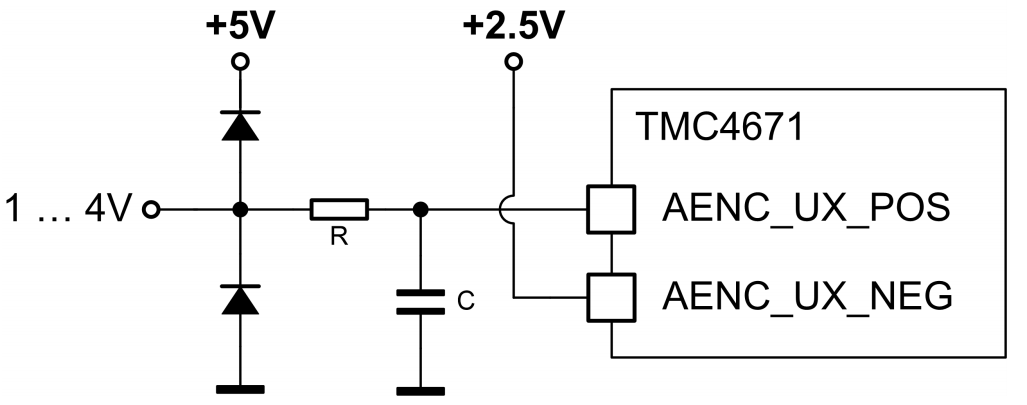
\includegraphics[width=0.5\textwidth]{graphics/Schema_Encoder_2_LP.png}
%	\caption{Teilschema aus Datenblatt TMC4671. Hier mit Shottky-Dioden anstelle IC.}
%	\label{fig:Schema_Encoder_2_LP}
%\end{figure}

%Die Widerstände \textbf{R703-R708} Stellen Spannungsteiler dar, welche gemäss Datenblatt eine benötigte Spannung von 2.5V bereitstellen.
%
%Der Kondensator \textbf{C703} ist ein Stützkondensator und dient der Speisung eines Ecoders. Die Versorgungsspannung wird jedoch nicht für den Resolver benötigt.
%
%Der Header \textbf{J6} ermöglicht, den Resolver an das PCB anzuschliessen.
%
%Abbildung \ref{fig:Schema_Encoder_LP} zeigt das Gesamte Schema mit den Komponenten, welche ein korrektes Einlesen des Resolvers ermöglichen.

%\begin{figure}[h!]
%	\centering	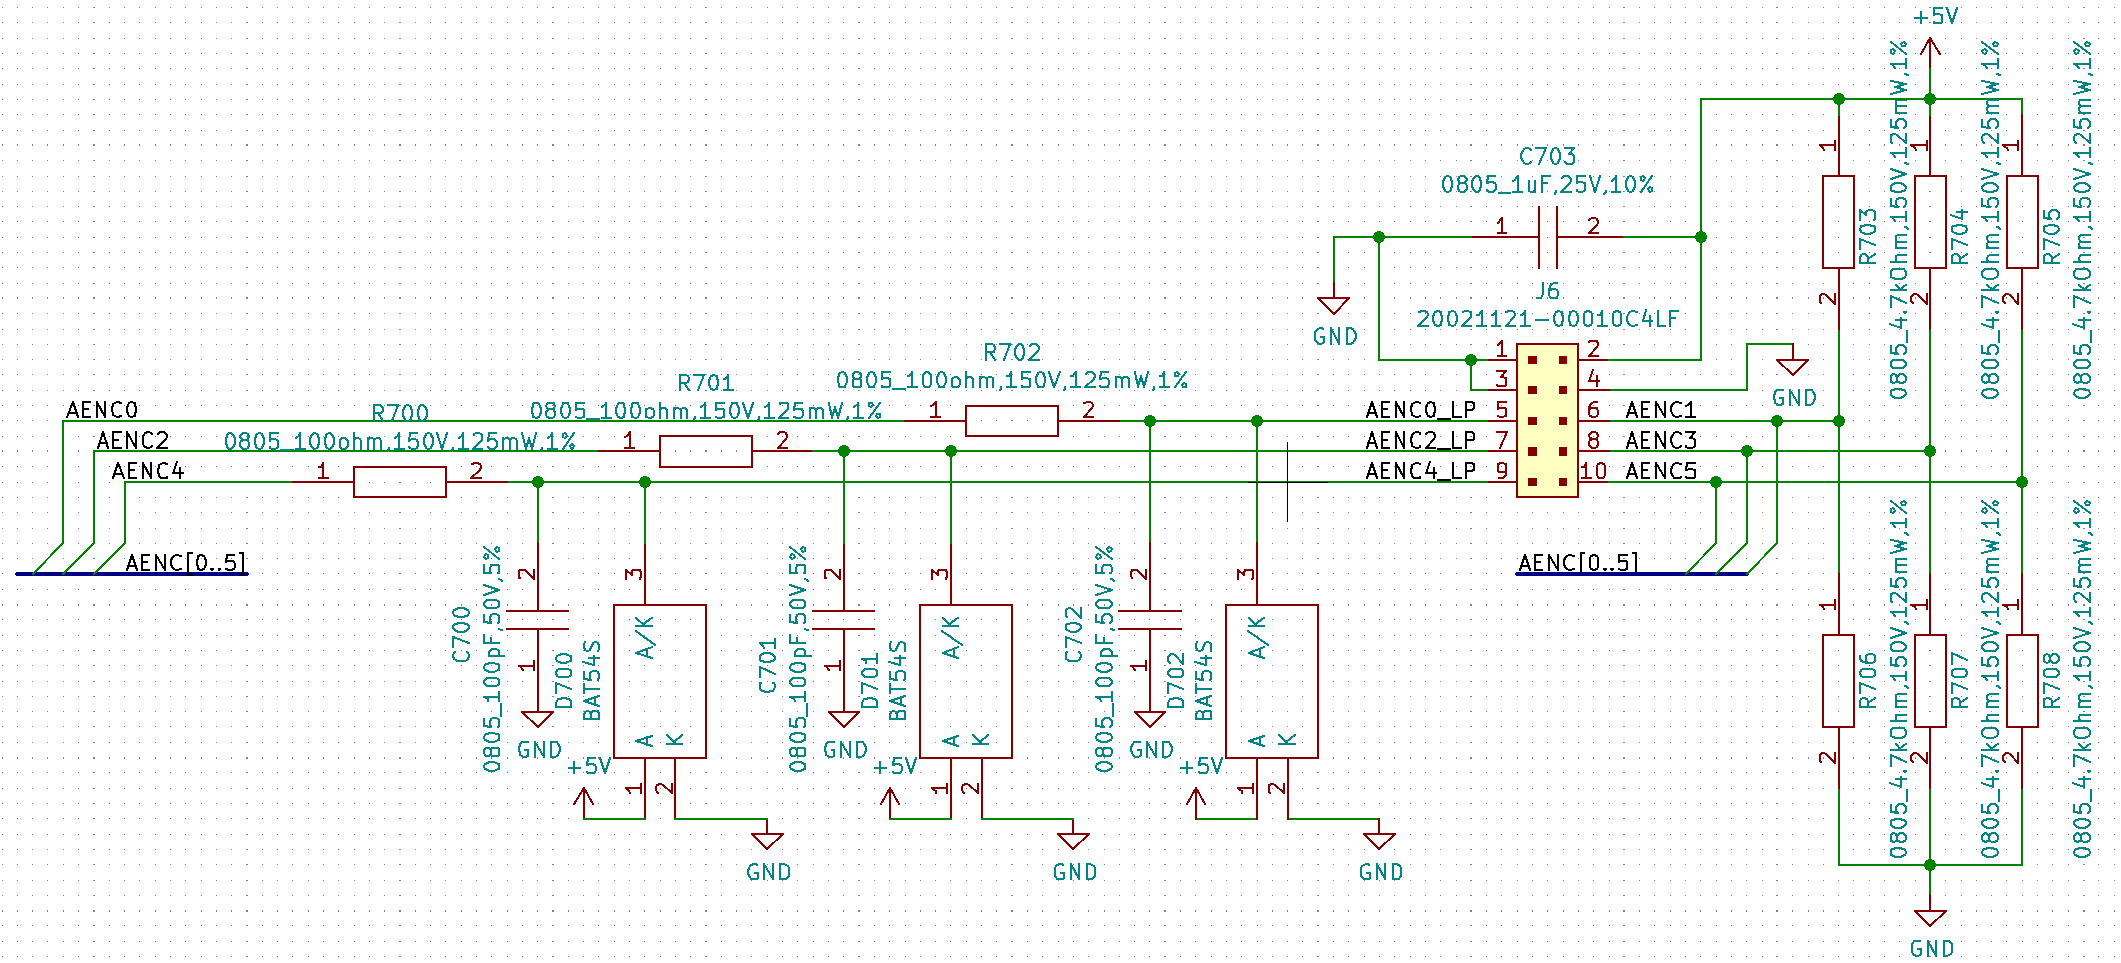
\includegraphics[width=\textwidth]{graphics/Schema_Encoder_LP.png}
%	\caption{Teilschema TMC4671. Hier Input Encoder.}
%	\label{fig:Schema_Encoder_LP}
%\end{figure}

%\subsubsection{Analog-Inputs}\label{subsubsec:Analog_Inputs}
%
%Auch hier wird das Eingangssignal mit einem Tiefpass gefiltert. Dafür werden die Widerstände R711 und R713 sowie die Kondensatoren C707 und C709 verwendet. Die Beschaltung und Dimensionierung wurde aus dem Datenblatt des TMC4671-EVAL-Board entnommen. Die Zeitkonstante des Filters beträgt gemäss Formel \ref{equ:Berechnung_Analog_LP} 400ns. Das Schaltungsprinzip ist in Abbildung \ref{fig:Schema_Analog_LP} dargestellt. \cite[PDF S.25]{trinamic_drawings_2018}
%\begin{equation}
%\tau = R \cdot C = 4\cdot 10^{3}\Omega \cdot 100\cdot10^{-12}F = 10 \cdot 10^{-9}s = 400ns
%\label{equ:Berechnung_Analog_LP}
%\end{equation}
%
%Weiter befindet sich ein zweiter Widerstand in jeder Schaltung
%\todo{Funktion zweiter Widerstand herausfinden.}
%
%Das letzte Bauteil, welches noch beschrieben werden muss, sind die Dioden D703 und D704. Diese stellen jeweils wieder einen Über- bzw. Unterspannungsschutz dar, um den Messeingang des TMC4671 zu schützen. Das Bauteil ist das selbe wie oben im Encoder-Teil, weshalb hier auf eine tiefere Beschreibung verzichtet wird.
%
%\begin{figure}[h!]
%	\centering	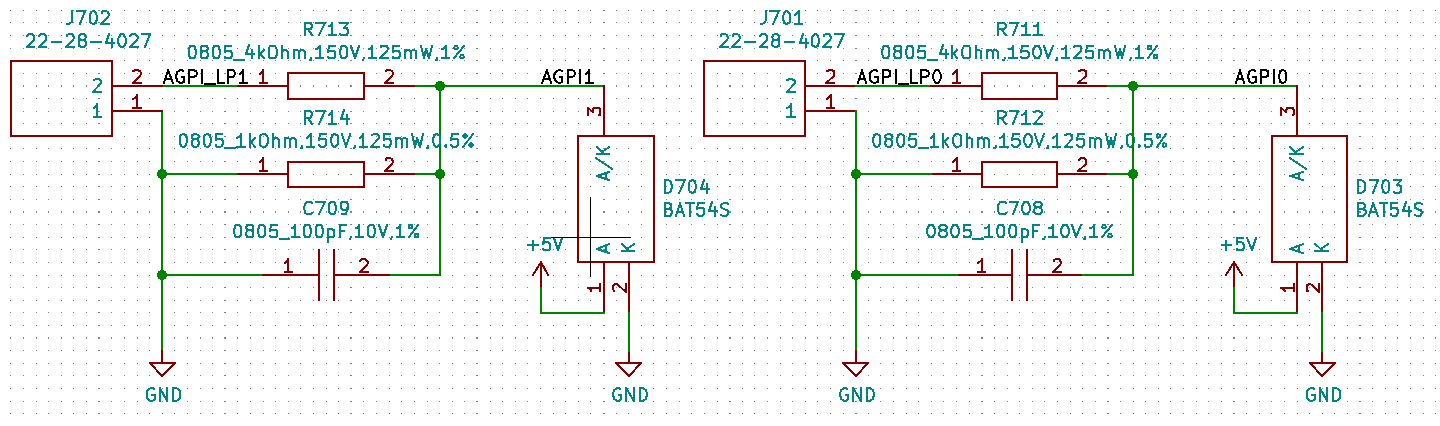
\includegraphics[width=0.8\textwidth]{graphics/Schema_Analog_Inputs_LP.png}
%	\caption{Teilschema TMC4671. Hier Inputs Analog.}
%	\label{fig:Schema_Analog_LP}
%\end{figure}
%
%
%\subsubsection{Motorspannung-Input}\label{subsubsec:Motorspannung_Input}
%
%\cite[PDF S.25]{trinamic_drawings_2018}
%\begin{figure}[h!]
%	\centering	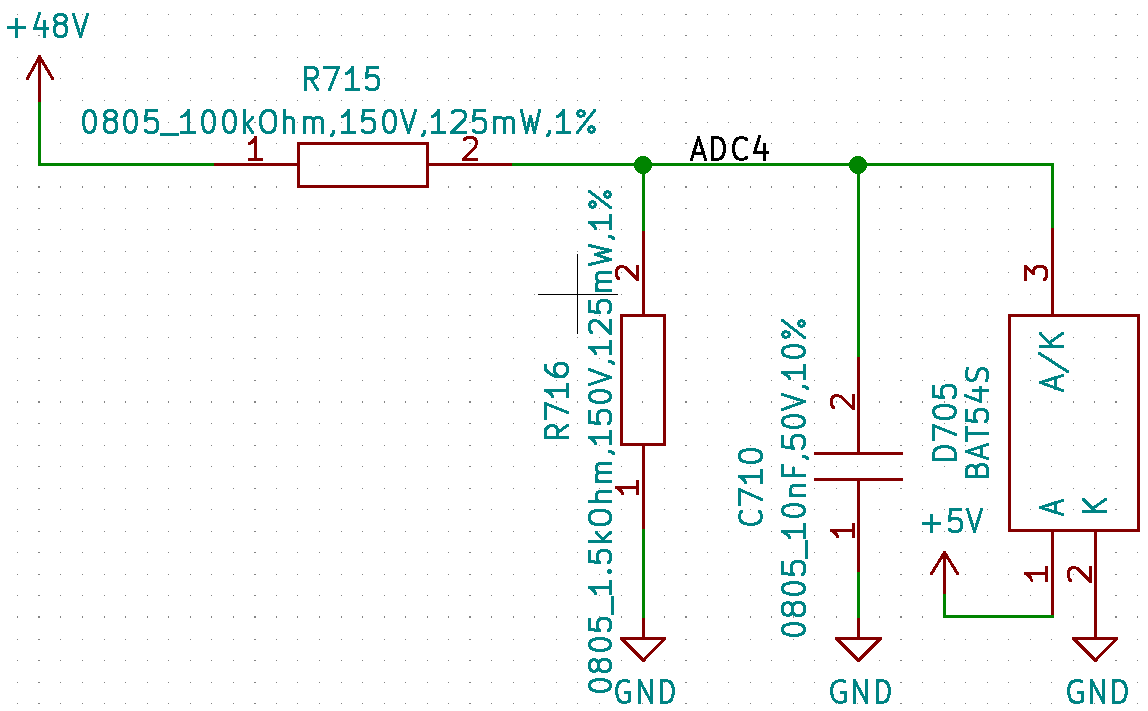
\includegraphics[width=0.45\textwidth]{graphics/Schema_VM_Input_LP.png}
%	\caption{Teilschema TMC4671. Hier Input Motorspannung.}
%	\label{fig:Schema_Encoder_LP}
%\end{figure}